 Median OS in the entire population treated with  CDK4/6 inhibitors was 46 months (95\%CI 39.4–55.6). Median PFS  was 20.3 months (95\%CI 18.3–24.2). The median OS in the entire population after removing abemaciclib changed very little.
Following this, we compared Palbociclib and riboclib as first line treatment. We found that regarding OS, there is no significant difference among the two, but ribociclib is significantly better in terms of PFS (p-value $\le$ 0.001) (figure \ref*{fig:interest}).
We did 


\begin{figure}[ht]
  \caption{Survival curves for Palbociclib and Ribociclib (1st line) - Progression Free Survival and Overall Survival}\label{fig:interest} 
  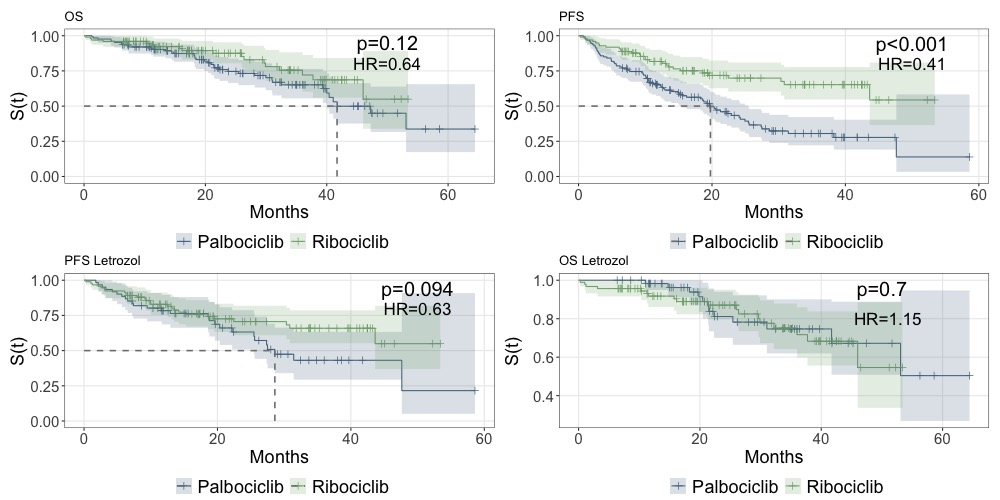
\includegraphics[scale=0.4]{figures/interest_curve_both.jpeg}%

\end{figure}


We then compared both with a cox regression, checking that the trend seen in figure  \ref{fig:interest} continues where OS shows no significant difference between palbociclib and ribociclib but a significantly better PFS for ribociclib (figure \ref*{tab:cox}). When adjusted to Stage, visceral metastases, Age and ECOG, ribociclib is associated to an HR of 0.44, implying that ribociclib as a first line treatment reduces the risk of the disease progression by $~$60\% compared to palbociclib as first line treatment. The proportional hazards assumption was confirmed with p values all over 0.10.
\begin{table}[ht]
  \centering
  \caption{Cox Regression with palbociclib and Ribociclib - Progression Free Survival and Overall Survival}\label{tab:cox} 
  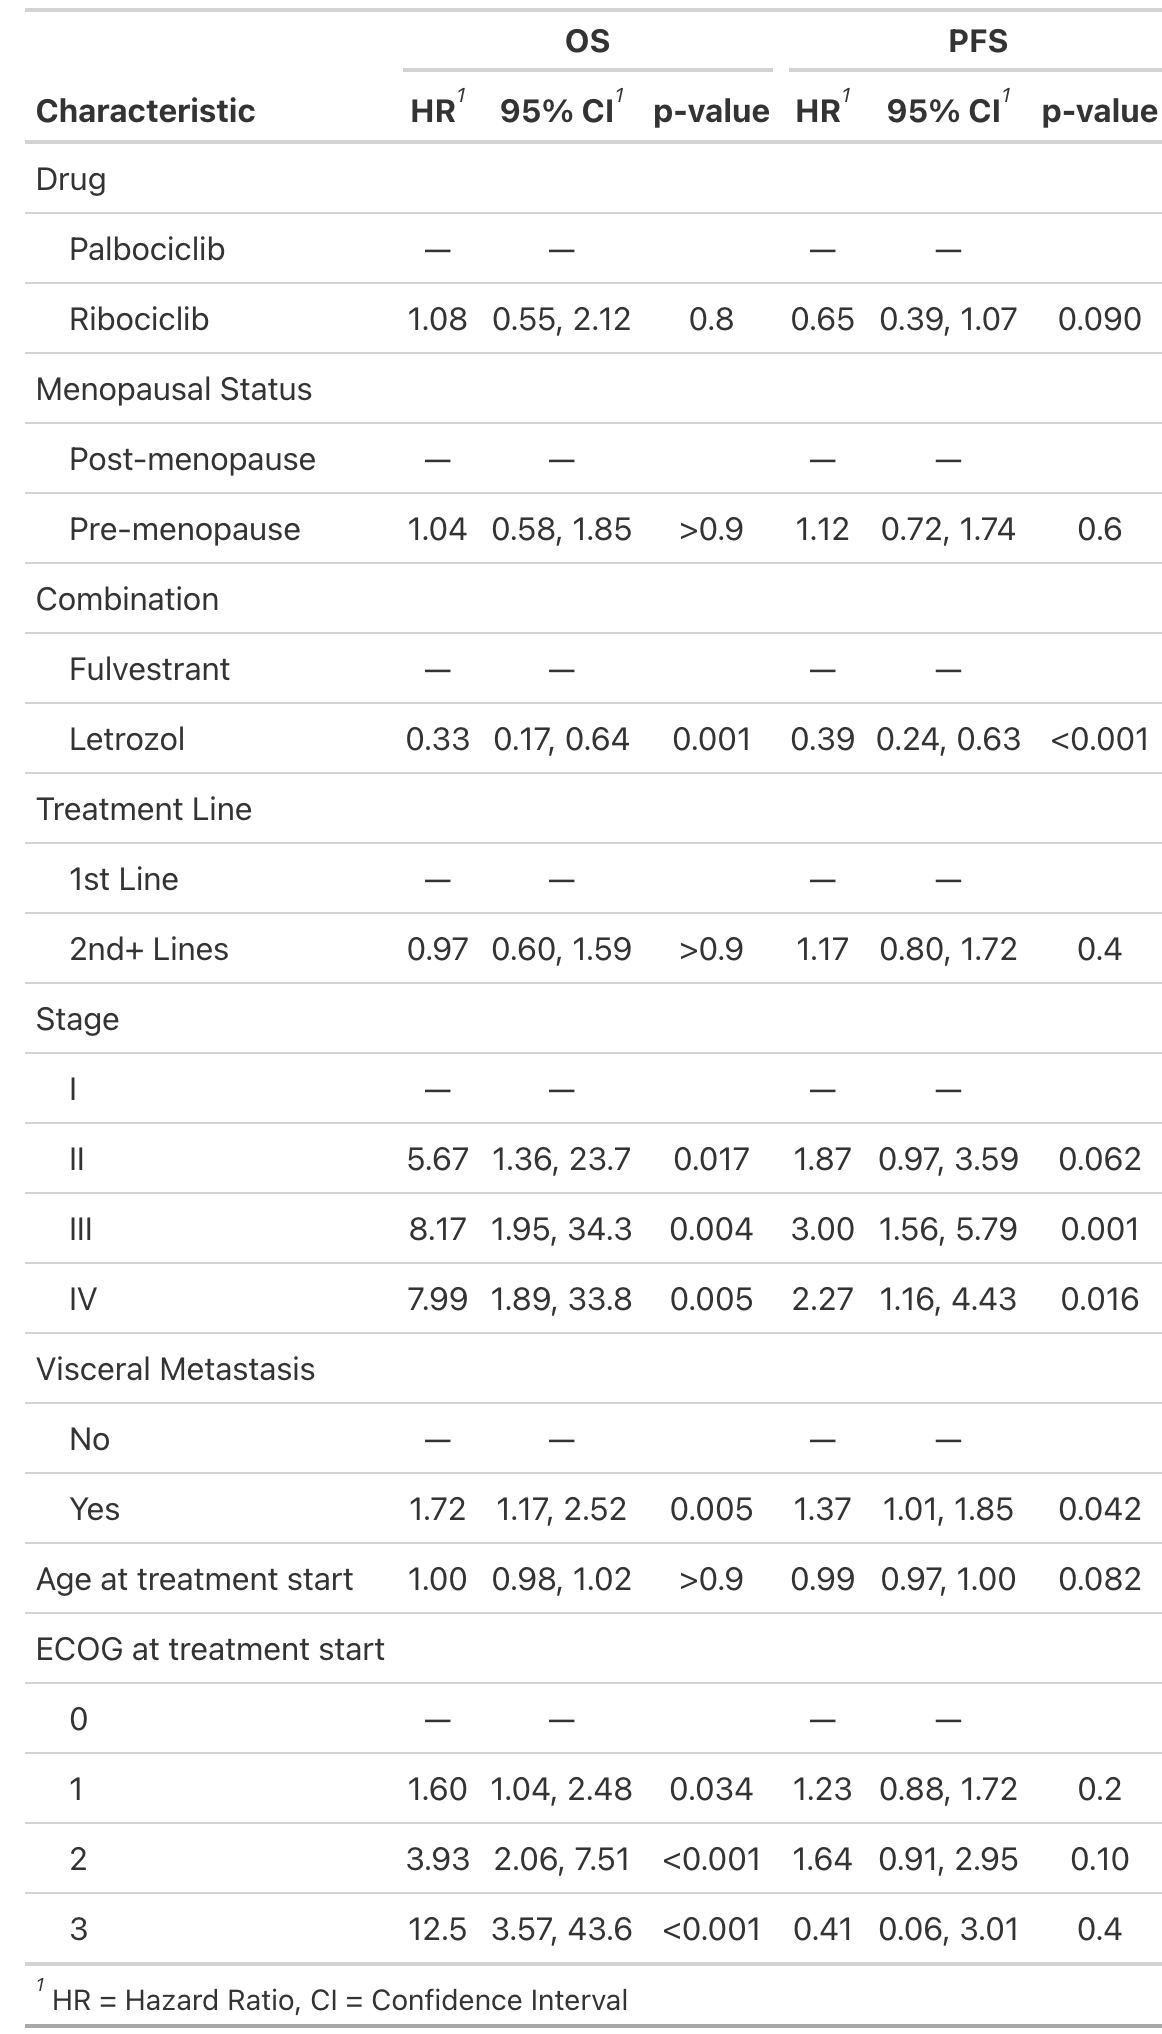
\includegraphics[scale=0.25]{figures/cox_both.png}%

\end{table}

When comparing endocrine therapy with CDK4/6 inhibitors as first line treatment, we see that only Ribociclib is significantly better in terms of PFS and OS (p-value $\le$ 0.001). When comparing palbociclib as first line, we see that there is no significant difference both in terms of PFS and OS (p=0.08 and 0.6)
(figure \ref*{fig:grouped}).
\begin{figure}[ht]
  \centering

  \caption{Survival curves (OS and PFS) comparing endocrine therapy (ET) to CDK4/6 inhibitors as 1st line. p values shown as pairwise vs HT. }\label{fig:grouped} 
  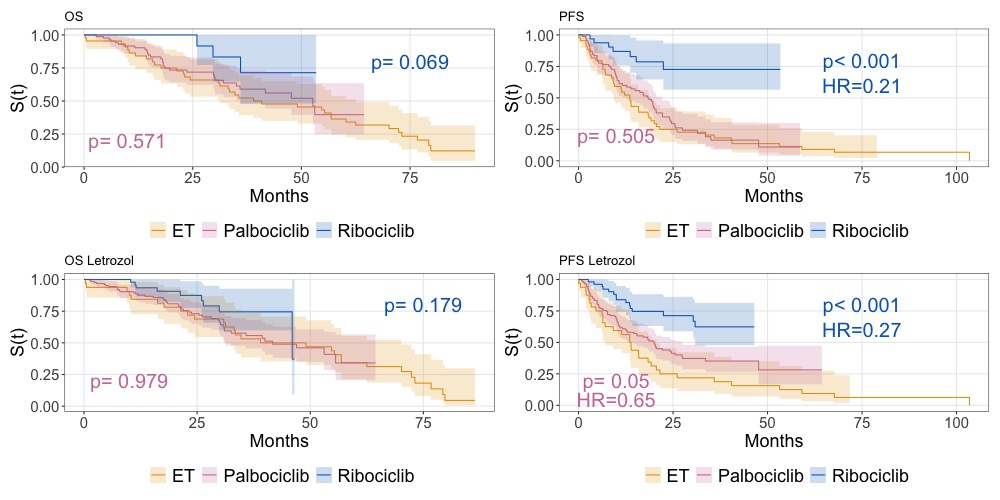
\includegraphics[scale=0.4]{figures/grouped_curve_both.jpeg}%

\end{figure}

When comparing palbociclib and ribociclib adjusted for ATE weights, we found a different scenario from previous assessments. There is a significant difference between the two in terms of OS and PFS (figure \ref*{fig:propensity}). We calculated the weights taken into account stage, age at treatment start, treatment line and ECOG.

\begin{figure}[ht]
  \centering

  \caption{Comparison of palbociclib and ribociclib survival curves adjusted for propensity scores  }\label{fig:propensity} 
  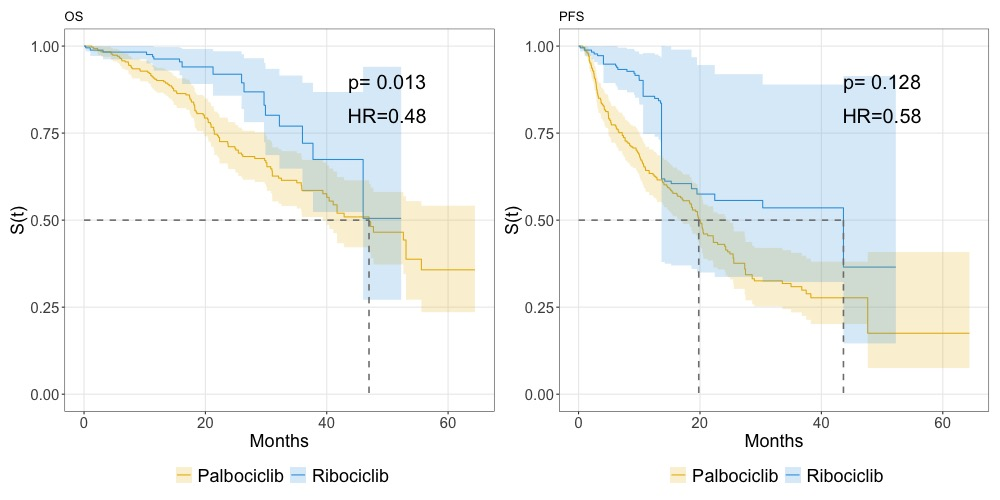
\includegraphics[scale=0.35]{figures/propensity_score_both.jpeg}%

\end{figure}

The Cox regression adjusted for weigths shows that ribociclib is associated to an HR of 0.47 [0-26-0.87], implying that ribociclib reduces the risk of the death by $\sim$50\%  compared to palbociclib. The HR for PFS is 0.44 [0.26-0.62], implying that ribociclib reduces the risk of the disease progression by $\sim$60\% compared to palbociclib, which also indicates the adjustment caused little to no effect on the results (figure \ref{fig:cox}). Proportional hazards assumptions confirmed as well.